\section{Konzeption und Planung des Systems}
\subsection{Aufbau des Systems}
\subsubsection{Architektur}
Das System besteht aus drei verschiedenen Komponenten, dem Quellsystem, einem Extraktor sowie einem Zielsystem. Im Quellsystem befinden sich die Rohdaten aus dem operativen Betrieb. Diese sollen mit Hilfe des Extraktors extrahiert und im Zielsystem strukturiert abgespeichert werden. Während es sich beim Quellsystem um eine Jira Cloud-Instanz handelt, ist das Zielsystem eine NoSQL-Datenbank. Der Extraktor ist ein Softwareprogramm, welches periodisch zur Ausführung gebracht wird.
\subsubsection{Konzept des Data Warehouses}
Die Architektur unseres Systems ist einem Data Warehouse sehr ähnlich und erfüllt alle Eigenschaften eines Data Warehouses nach Inmon. Diese Erkenntnis unterstützt beim Entwurf des Systems und ermöglich es, Konzepte, Best Practices und Technologien im Zusammenhang mit dem Data Warehouses einzusetzen.
\begin{itemize}
  \item Historisierung: Alle Objekte des Jira Systems sind mit einem Zeitstempel der letzten Änderung, sowie der Erstellung versehen, was den Aufbau eines historisierten Datenbestandes ermöglicht.
  \item Integriert: Wir extrahieren unsere Daten aus nur einem System. Das Hinzufügen eines weiteren Jira-Systems ist möglich und wird in der Architektur des Systems berücksichtigt.
  \item Nicht-Volatilität: Der Datenbestand wird dauerhaft aufgebaut und bleibt bestehen. In Gegensatz zu operativen Systemen werden aus unserem Zielsystem keine Daten gelöscht.
  \item Fach-orientiert: Unser Datenbestand hält fachliche Daten aus dem operativen Geschäftsablauf.
\end{itemize}
[ZITAT]\\\\
Der Aufbau des Systems und dessen Komponenten sind angelehnt an bereits existierende Referenzmodelle für Data Warehouses. Der Datenbestand des Data Warehouse soll mit hilfe eines ETL-Prozesses aufgebaut werden. Dabei werden Daten aus einem Jira-System (Quellsystem) extrahiert, transformiert und dann in die Graphdatenbank (ArcadeDB) geladen. Außerdem gibt es ein Metadaten-Repository, um Daten über den Extraktionsprozess und dessen Daten zu speichern. Dieses Metadaten-Repository wird unter anderem dazu dienen die genauen Ausführungszeiten, sowie die Token der Texte. Abbildung 1 gibt einen vereinfachten Überblick über das System und dessen Komponenten.
\begin{figure}[h]
\centering
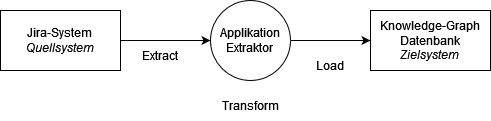
\includegraphics[scale=.6]{dateien/ETL-Prozess.jpg}
\caption{Der ETL-Prozess zum Aufbau des Knowledge Graphen}
\label{fig:meine-grafik}
\end{figure}
\subsection{Anforderungserhebung}
Um die gesamte Applikation und und dessen Komponenten besser zu verstehen und bessere Anforderungen formulieren zu können, betrachten wir dieses als System. Die einzelnen Bestandteile wiederum können jeweils als Subsystem bezeichnet werden. Ist unser System mit einem externen System integriert, so wird dieses als Umsystem bezeichnet. In unserer Architektur entspricht das Jira-System einem Umsystem. Als Subsystem werden alle Beständeteile betrachtet, welche dem System vollständig angehören. Die Graph-Datenbank, der Jira-Extraktor und eine Datenbank zur Speicherung von Konfigurations- sowie Metadaten wären somit Subsysteme. [978-3-658-37194-4, S.60] \\
Zunächst müssen die Anforderungen an das System erhoben und kategorisiert werden. Dabei wird zwischen funktionalen und nicht-funktionalen Anforderungen unterschieden. Alle in diesem Kapitel erhobenen Anforderungen sind so gestaltet, dass die Applikation im beliebigem Kontext  und dynamisch eingesetzt werden kann. Den Anforderungen liegt kein spezifischer Anwendungsfall zugrunde.\\
Es gibt vier verschiedene Ansätze zur Erfassung für Anforderungen. Die folgenden Anforderungen wurden alle auf Basis eigener Überlegungen und ersten Code-Ausführungen durch den Ansatz "Kreativität" erhoben. Für eine Beobachtung oder das Untersuchen von Artifakten sind keine Ressourcen wie z.B. Dokumente oder bereits bestehende Anforderungen verfügbar.[978-3-658-37194-4, S.60]. \\
Jeder Stichpunkt beschreibt eine Anforderung an das System, einer Komponente des Systems oder einen Ablauf im System und wird nach einem bestimmten Schema formuliert. Einer Anforderung kann eine bestimmte Verbindlichkeit zugeordnet werden, welche durch die Formulierung der Anforderung deutlich wird. Muss eine Anforderung umgesetzt werden, so hat diese die höchste Priorität und ist für die grundlegende Fertigstellung der Applikation unerlässlich. Soll eine Anforderung umgesetzt werden, so schafft diese einen deutlichen Mehrwert und verbessert die Applikation signifikant. Kann eine Anforderung umgesetzt werden, so handelt es sich dabei um eine optionale Erweiterung, welche nur umgesetzt wird, wenn die notwendigen Resourcen verfügbar sind.\\
Im Anschluss an die Anforderungserhebung werden die Randbedingungen durch einen Vergleich von verschiedenen Technologien festgelegt.
\subsubsection{Funktionale Anforderungen}
Funktionale Anforderungen beschreiben die fachliche Spezifikation eines Systems, sowie alle Schnittstellen inklusive der Eingangs- sowie Ausgabeparameter des Systems. Diese Anforderungen werden in der Testphase der Entwicklung in Testfälle überführt. Können die Tests erfolgreich ausgeführt werden, so erfüllt die Applikation die zuvor festgelegten Anforderungen.\\
Folgende funktionale Anforderungen müssen erfüllt sein:
\begin{itemize}
  \item Das System muss genau eine Jira-Cloud Instanz als Datenquelle verwenden. 
  \item Die Interaktion mit der Jira-Cloud API in Java soll mittels der breits von Atlassian bereitgestellten Dependencies umgesetzt werden. Es soll Basic-Authorization verwendet werden. Als Java Build-Tool soll Maven verwendet werden.
  \item Es soll möglich sein, diese Projekte genau zu konfigurieren. Dabei soll es auch möglich sein, für jedes Projekt die zu extrahierenden Vorgangstypen festzulegen. Der Speicherort zu dieser Konfigurationsdatei muss durch Umgebungsvariablen dynamisch konfigurierbar sein. Folgende JSON-Datei gibt unserer Applikation die Anweisung, den Issuetype Task und Bug des Projektes mit dem Schlüssel KAW und den Issuetype Story und Task des Projektes mit dem Schlüssel MUN zu extrahieren und in das Zielsystem zu laden:
    \begin{minted}{json}
    {
        "KAW": ["Task", "Bug"],
        "MUN": ["Story", "Task"]
    }
    \end{minted}
  \item Das System muss dynamisch durch das Konfigurieren der Datenbankverbindung mittels Umgebungsvariablen an die Zieldatenbank angebunden werden. Dabei muss der Name und das Passwort des Benutzers, sowie der Host, der Port und das Schema der Datenbank konfiguriert werden können.
  \item Das System soll beim extrahieren eines Jira Tickets und eines Jira Subtasks erkennen, ob ein Duplikat vorliegt und beim einfügen in die Zieldatenbank eine Verknüpfung herstellen, welche eine Aussage trifft, wie ähnlich beide Objekte sind.\\
  Um die Duplikatprüfung durchzuführen soll das System auf die Schlüsselwörter zurückgreifen, welche sich in den relevanten Werten von Attributen eines Objektes befinden. Teil dieser Attribute sind beispielsweise der Titel oder die Beschreibung eines Tickets.
  \item Die Applikation muss den ETL-Prozess beim Start der Anwendung durchführen und nach Beendigung des ETL-Prozess mit einem Fehlercode terminieren.
  \item Das System soll nicht eigenständig die zeitliche Ausführung terminieren sondern von seiner Umgebung zur Ausführung gebracht werden. Beispielsweise kann die Terminierung in einem Kubernetes Cluster stattfinden. Ein Vorteil wäre, dass in diesem Fall mehrere Knoten zur Verfügung stehen, welche eine höhere Ausfallsicherheit garantieren. Des weiteren haben sich externe Scheduling-Methoden im Gegensatz zur selbständigen Implementierung als sehr zuverlässig erwiesen. \\
  \item Das System soll alle neuen oder geänderten Objekte periodisch exportieren. Ein Exportvorgang soll einmal pro Tag stattfinden. Ein Exportvorgang soll immer zur gleichen Tageszeit und außerhalb der Zeit geschehen, in welcher mit dem Zielsystem gearbeitet wird.
  \item Das System soll alle relevanten Objekte exportieren, die ein Jira-Projekt umfassend beschreiben. Diese sind z.B. Vorgänge, Vorgangstypen, Projekte und Kommentare.
  \item Das System muss alle Daten auf die Zieldatenbank transformieren. Alle für die Analyse nicht relevanten Metadaten aus dem Jira-System sollen aussortiert werden. Ausschließlich wichtige Felder für die folgende Analysen sollen in ein angemessenes Format transormiert werden.
  \item Die Extraktion eines jeden Objektes soll dokumentiert werden. Hierzu werden alle Vorgänge in einer Datenbank erfasst. Zu jedem Vorgang werden mindestens der Zeitpunkt, der Typ und die Kennung eines Objektes erfasst.\\
  Falls bei einem Teilvorgang der Extraktion ein Fehler auftritt und das zugehörige Objekt nicht extrahiert und geladen werden kann soll ein Log-Eintrag bezüglich des Objekts in strukturierter und maschinenlesbarer Sprache erzeugt werden. Dies ermöglicht in Zukunft eine weitere Fehlerbehandlung.
  \item Die Applikation muss Änderungen an Objekten erkennen und diese historisieren, also alle Änderungen in einen zeitlichen Zusammenhang bringen und ordnen können.
\end{itemize}

Folgende funktionale Anforderungen sollen erfüllt sein:
\begin{itemize}
  \item Die Zieldatenbank soll für effiziente Analysen geeignet sein und Objekte effizient miteinander verknüpfen. Dadurch sollen möglichst schnell Verknüpfungen sowie ein Kontext hergestellt werden können.
  \item Die Zieldatenbank soll für sehr große Datenmengen konzipiert sein, da alle Objekte versioniert werden und somit mehrfach speichern werden.
\end{itemize}
Folgende funktionale Anforderungen können erfüllt sein
\begin{itemize}
  \item Der Extraktor kennt für jeden Extraktionsvorgang sowie den Gesamtvorgang die benötigte Zeit und speichert diese für spätere Analysen.
\end{itemize}
\subsubsection{Nicht-funktionale Anforderungen}
Nicht-funktionale Anforderungen beschreiben den Aufbau des Systems. Auch sie werden in Form von Testfällen nach Beenden der Entwicklung geprüft und müssen für eine erfolgreiche Entwicklung erfüllt sein.\\
Folgende nicht-funktionale Anforderungen müssen erfüllt sein:
\begin{itemize}
\item Das System muss alle Extraktionsvorgänge in einer Datenbank dokumentieren und falls eine Ausführung nicht stattgefunden hat, dieses erkennen, diese bis zu einem gewissen Zeitpunkt nachholen. Eine Ausführung kann beispielsweise nicht stattfinden, wenn das System zum geplanten Zeitpunkt nicht lauffähig ist. Wird die Applikation später gestartet, soll diese mit der Ausführung beginnen.
\item Das Systen muss weitestgehend fehlerfrei arbeiten. Insbesondere müssen alle vorgesehenen Objekte extrahiert werden. Es darf kein Objekt, welches geändert oder neu erstellt wurde ohne Export im Quellsystem (durch z.B Fehler mit dem Zeitstempel durch Latenzen bei der Anfrage) verbleiben.
\item Das System muss eine hohe Fehlertoleranz aufweisen und verschiedene Mechanismen implementieren, welche eine hohe Resilienz des Systems gewährleisten. Falls in einem Extraktionsvorgang eine Ausnahme auftritt, so muss durch einen Logeintrag erkennbar sein, bei welchem Objekt und Objekttyp oder Jira-Schnittstelle diese verursacht wurde. Ein weiterer Versuch, das entsprechende Objekt zu extrahieren, soll beim nächsten regulären Extraktionsvorgang angestoßen werden.
\item Das System muss flexibel gestaltet sein und alle notwendigen Parameter zur Extraktion durch Umgebungsvariablen erhalten. Wichtige Parameter sind beispielsweise der Jira Benutzer, dessen Passwort und die URL der Jira Instanz. Ein Pfad zur Konfigurationsdatei aller relevanten Jira-Projekte sowie Vorgangstypen, welche zur Extraktion bestimmt sind, soll auch durch eine Umgebungsvariable gesetzt werden können.
\item Die Applikation muss speziell für containerisierte Umgebungen und Cloudumgebungen bestimmt sein und somit als Image für IaC-Anwendungen (z.B. Docker oder Kubernetes) ausführbar sein.
\end{itemize}
Folgende nicht-funktionale Anforderungen sollen erfüllt sein:
\begin{itemize}
  \item Der Extraktor soll nicht skalierbar sein. Es ist nur eine Instanz für jeweils einen Extraktionsvorgang vorgesehen. Ein Entwurf, um das System als Cluster zu betreiben ist sinnvoll, wird aber aufgrund von übermäßigem Aufwand bei der Implementierung der Kommunikation zwischen Instanzen nicht umgesetzt. Die Zieldatenbank muss aber in der produktiven Umgebung als verteilte Datenbank kompatibel mit dem Extraktor sein.
  \item Die Applikation soll möglichst intuitiv konfiguriert werden können und durch möglichst wenig Umgebungsvariablen konfiguriert werden können.
\end{itemize}
Es werden keine Anforderungen an die Extraktionsdauer gestellt. Dies ergibt sich daraus, dass die Applikation als Hintergrundprozess ausgeführt wird und durch einen langen ETL-Prozess kein Anwender beeinträchtigt wird. Primäres Ziel der Applikation ist die Extraktion und Aufbereitung von fachlich korrekten und konsistenten Daten. Außerdem ist vorgesehen, die Anwendung gezielt auszuführen, wenn möglichst keine Anwender mit dem System interagieren. Ressourcen zur Optimierung der Ausführungsdauer werden daher gezielt eingesetzt, um die Fehlerfreiheit der Applikation zu verbessern.
